\subsection{Уравнение Бернулли}
За время $\Delta t$ жидкость течет из сечения: \(1 \to  1' \text{ и } 2 \to 2'\) (см. рис. \ref{fig:8.1.2}).

Запишем теорему об изменении механической энергии.
\[d \, W_{\text{механическая}} = d \, A^{\text{давления}}\]
\[\frac{d \, m}{2}(v_2^2 - v_1^2) + g(h_2 - h_2) d \, m = v_1 p_1 d \, S_1 \cdot d \,t_1+v_2 p_2 d \, S_2 \cdot d \,t_2\]
\[\begin{aligned}
	d m = \rho_1 v_1 d S_1 \cdot d t && &&  v_1 dS_1 = v_2 dS_2
\end{aligned}\]
\[\begin{aligned}
	\frac{\rho v_1^2}{2} + \rho g h_1 + p_1 = \frac{\rho v_2^2}{2} + \rho gh_2 + p_2 && \Rightarrow && \boxed{\frac{\rho v^2}{2} + \rho g h + p = const}
\end{aligned}\]

\textbf{Обобщение:} Выполняется вдоль линии тока\footnote{Линия тока -- линия, касательная которой в каждой точке совпадает с вектором движения}.
\begin{figure}[h]
	\centering
	\begin{minipage}{0.49\linewidth}
		\centering
		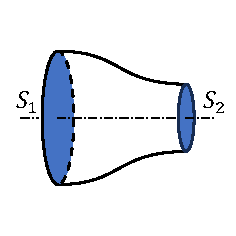
\includegraphics[width=0.7\linewidth]{image/Уравнение Бернули 2.pdf}
		\subcaption{ }
		\label{fig:8.1.1}
	\end{minipage}
	\hfill
	\begin{minipage}{0.49\linewidth}
		\centering
		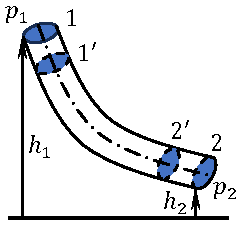
\includegraphics[width=0.7\linewidth]{image/Уравнение Бернули.pdf}
		\subcaption{ }
		\label{fig:8.1.2}
	\end{minipage}
	\caption{Пример уравнения Бернулли}
	\label{fig:bernoulli}
\end{figure}

\textbf{Пример:} (см. рис. \ref{fig:8.1.1})
\[\begin{aligned}
	\frac{\rho v_1^2}{2} + p_1 = \frac{\rho v_2^2}{2} + p_2 && (h = const)
\end{aligned}\]

Так как $S_1 > S_2$, то $v_1 < v_2$ и поэтому $p_1 > p_2$.